\documentclass[conference]{IEEEtran}
\usepackage[utf8]{inputenc}
\usepackage{amsmath,amssymb,graphicx,booktabs}

\usepackage[hidelinks,unicode,pdftitle={How Many Validation Items Does Merge-Coefficient Selection Need? Selection Regret on Qwen2.5-0.5B Interpolations (ARC, HellaSwag, WinoGrande)},pdfauthor={Dheiver Francisco Santos},pdfkeywords={model merging, validation set size, selection regret, Qwen2.5, evaluation},pdfsubject={Preprint, Figshare, doi:10.6084/m9.figshare.35014009}]{hyperref}
\begin{document}

\title{How Many Validation Items Does Merge-Coefficient Selection Need? Selection Regret on Qwen2.5-0.5B Interpolations (ARC, HellaSwag, WinoGrande)}

\author{\IEEEauthorblockN{Dheiver Francisco Santos, PhD}
\IEEEauthorblockA{Independent Researcher\\
Maceió, Alagoas, Brazil\\
ORCID: https://orcid.org/0000-0002-8599-9436\\
Preprint, Figshare, 2026, \href{https://doi.org/10.6084/m9.figshare.35014009}{doi:10.6084/m9.figshare.35014009}, CC BY 4.0}}

\maketitle

\begin{abstract}
How large must the validation set be when selecting a merge coefficient? We take an 11-point linear-interpolation grid between Qwen2.5-0.5B and its Instruct variant, scored by the macro average of four multiple-choice benchmarks. We measure selection regret (test accuracy of the best grid point minus that of the selected point) on random validation subsets of $n\in\{30,60,100,200\}$ items per task, 1000 draws each, from a pool of about 300 items per task. The mean regret is $0.50$, $0.53$, $0.51$ and $0.50$~pp. We detect no trend, and the pre-registered hypothesis that regret falls with $n$ is not supported. Selection does not change the expected regret, although the probability of zero regret roughly doubles ($0.10$ to $0.20$). The probability of beating both originals ($0.31$--$0.37$) is of the same order as that of a random pick ($0.36$), whose regret is $0.46$~pp. The test accuracies of all 11 points lie within $1.06$~pp; we conjecture that this flatness sets the regret. One model pair, one grid, one pool.
\end{abstract}

\begin{IEEEkeywords}
model merging, validation set size, selection regret, Qwen2.5, evaluation
\end{IEEEkeywords}

\section{Introduction}
Model-merging recipes select coefficients with a validation set whose size is usually dictated by convenience: the evaluation of each candidate costs a forward pass over all validation items, and the grid can have dozens of points. A practitioner then asks whether fewer items would do, or whether more are needed. The standard statistical answer is that the standard error of an accuracy shrinks as $1/\sqrt{n}$. Whether two candidates can be resolved then depends on their true difference relative to that error \cite{miller2024errorbars}. When candidates differ by well under one point, a few hundred items do not resolve them. The interesting quantity is then not the error of each score but the cost of picking the wrong candidate.

We therefore measure \emph{selection regret}: how much test accuracy is lost, relative to the best grid point, by choosing with a validation subset of $n$ items per task. The experiment reuses the item-level outcomes of the 11-point base-to-instruct interpolation of Qwen2.5-0.5B \cite{qwen2024qwen25}, so in the main analysis no model is evaluated again, and the validation subsets differ only in which items are seen.

\textbf{Contributions.} (i) Selection regret as a function of $n$ on a real merge grid, with the probability of beating both original models. (ii) A random-choice reference and the range of the test curve, which together show how much of the regret the validation set can possibly remove here. (iii) An explicit statement of what the $n=300$ point is and is not.

\section{Related Work}
\textbf{Sample size of evaluations.} Miller \cite{miller2024errorbars} recommends reporting standard errors for language-model evals; the lm-evaluation-harness \cite{gao2021lmeval} and benchmarks such as ARC \cite{clark2018arc}, HellaSwag \cite{zellers2019hellaswag} and WinoGrande \cite{sakaguchi2019winogrande} fix the item counts that practitioners actually have. Our quantity differs: it is the loss from a selection decision made at a given $n$, not the power to detect a difference. \textbf{Reusing a holdout.} The adaptive data analysis literature \cite{dwork2014adaptive}, from which reusable-holdout mechanisms come, studies how many adaptive queries a finite holdout can answer before its estimates stop being valid; we ask the dual question for one query over a grid of 11 candidates. \textbf{Distribution of benchmark scores.} Recht et al.\ \cite{recht2019imagenet} report that accuracies drop on newly collected test sets while the relative order of models is largely preserved, a reminder that a single pool is one draw; the bootstrap \cite{efron1979bootstrap} is the tool we use for intervals elsewhere in this study.

\textbf{Selecting merge ingredients and coefficients.} Model soups propose a greedy selection of ingredients by held-out accuracy \cite{wortsman2022soups}. Related recipes average weights of models fine-tuned on diverse data or rewards \cite{rame2022ratatouille,rame2023rewarded}; these describe weight averages, not selection. In task-vector methods, scaling coefficients are hyperparameters \cite{ilharco2022taskarithmetic,yadav2023ties}. Evolutionary and Bayesian searches optimize merge recipes or checkpoint-merging weights against a development metric \cite{akiba2024evolutionary,liu2024checkpointbo}. Alternative weightings (Fisher information) or learned coefficients (AdaMerging) have also been proposed \cite{matena2021fisher,yang2023adamerging}, as has composition of low-rank adapters with a few examples \cite{huang2023lorahub}. Surveys organize the methods \cite{yang2024survey}. We did not find a measurement of how the quality of the selected merge varies with the number of validation items on a small language-model grid. This paper measures it on one controlled grid and finds that, here, it does not vary detectably.

\textbf{Author's related work.} The author's technical notes cover neighboring topics in language-model training: model merging for capability composition \cite{santos2026modelmergingfo}, knowledge distillation and self-distillation \cite{santos2026knowledgedisti}, parameter-efficient fine-tuning (LoRA, QLoRA, DoRA) \cite{santos2026parametereffic}, mixture-of-experts training and sparse upcycling \cite{santos2026mixtureofexper}, curriculum learning and data-efficient pretraining \cite{santos2026curriculumlear}, synthetic data generation and self-improvement \cite{santos2026syntheticdatag}, and direct preference optimization \cite{santos2026directpreferen}. This paper instead reports a controlled held-out measurement. In a different domain, the author's JEPA preprint \cite{santos2026collapseresist} uses a similar controlled-comparison style (identical budgets, several seeds, confidence intervals).

\section{Method}
Let $\theta_t=(1-t)\theta_{\text{base}}+t\,\theta_{\text{inst}}$ for $t\in\mathcal{T}=\{0,0.1,\dots,1\}$. Let $A(t)$ be the macro test accuracy (four tasks, equal weight) and $V_S(t)$ the macro accuracy on a validation subset $S$ that contains $n$ items from each task.

\subsection*{Equations and their meaning}
\begin{align}
\hat t_S&=\arg\max_{t\in\mathcal{T}} V_S(t),\qquad A^\ast=\max_{t\in\mathcal{T}}A(t),\\
\mathrm{reg}(S)&=A^\ast-A(\hat t_S),\qquad \overline{\mathrm{reg}}(n)=\mathbb{E}_{S}\,\mathrm{reg}(S).
\end{align}
Eq.~(1) selects the coefficient that looks best on the subset (ties go to the smallest $t$, up to floating-point tolerance) and defines the best achievable test accuracy on the grid. Eq.~(2) is the selection regret: how many points of accuracy are lost by trusting the subset; it is zero only when the subset picks the test optimum. The expectation is over random subsets and is estimated by $1000$ draws. Two companions are
\begin{align}
P_{\mathrm{win}}(n)&=\Pr_S\!\big[A(\hat t_S)>\max\{A(0),A(1)\}\big],\\
\overline{\mathrm{reg}}_{\mathrm{rand}}&=A^\ast-\tfrac1{|\mathcal{T}|}\textstyle\sum_{t}A(t).
\end{align}
Eq.~(3) is the probability that the selected merge beats both original models on the test set. Eq.~(4) is the regret of picking a grid point uniformly at random, which needs no validation data and is the natural reference. Finally, since $0\le \mathrm{reg}\le \mathrm{range}:=A^\ast-\min_t A(t)$, the regret cannot exceed the range of the test curve, which is why we report that range.

\section{Experimental Protocol}
\textbf{Models.} Qwen2.5-0.5B and Qwen2.5-0.5B-Instruct \cite{qwen2024qwen25} (Apache-2.0); Hub commits in \texttt{MANIFEST.json} (base \texttt{060db64}, instruct \texttt{7ae5576}). Interpolation in fp32 on CPU, copy to bf16.

\textbf{Data and splits.} ARC-Easy and ARC-Challenge \cite{clark2018arc} (official validation/test), HellaSwag \cite{zellers2019hellaswag} and WinoGrande \cite{sakaguchi2019winogrande} (validation sets partitioned into disjoint validation and test parts, seed 0). Validation pool: 300 items per task (299 for ARC-Challenge). Test: 1000 per task (967 WinoGrande), 3967 items. Scoring: multiple-choice log-likelihood in the harness style \cite{gao2021lmeval}; HellaSwag length-normalized per character, WinoGrande partial scoring without normalization. All per-item outcomes are cached; subsets only re-index them.

\textbf{Selection.} For $n\in\{30,60,100,200\}$, 1000 random subsets of $n$ items per task are drawn \emph{without} replacement from the pool of 300 (seed 0), and the coefficient is selected on each subset. For $n=300$ the subset is the whole pool, so the experiment has no randomness: it is one deterministic realization. The test set is never used for selection; it is used only to score the selected coefficient and to define $A^\ast$.

\textbf{Baselines.} The two original models ($t=0$ and $t=1$), and a coefficient drawn uniformly from the grid (Eq.~4). We also report the regret of always choosing $t=0$ or $t=1$, post hoc, as limiting cases.

\textbf{Statistics.} Bars and brackets for $n<300$ are the 2.5--97.5 percentiles of the per-draw regret (a spread across subsets, not a confidence interval of the mean). Monte Carlo standard errors of the means are about $0.01$~pp ($0.0104$--$0.0114$). Because all subsets are drawn from one pool of 300 items, draws overlap, and the spread underestimates the variation across independent validation sets (Sec.~VI). The hypothesis, pre-registered in \texttt{experiments/PREREG.md} before any merge was run, is that regret falls with $n\in\{30,60,100,200,300\}$. No test of the trend is reported because the pre-registered success criterion applies to articles~1--6; this study is secondary. As a replication check, \texttt{experiments/an\_art0809\_extra.py} redraws the subsets with a different draw order and the same seed (0). The pre-registration (\texttt{experiments/PREREG.md}) fixed 5,000 bootstrap resamples; the analysis used 2,000 for a single accuracy and 3,000 for paired differences (5,000 for per-block NLL differences, Articles~7 and 10). This article draws 1000 subsets per $n$. Apart from one paired comparison ($t=0.7$ versus $t=0$), it reports no p-values. Ties in the validation score are resolved by the smallest $t$ in the main analysis (\texttt{np.argmax}, which is exact only up to floating-point tolerance: with a tolerance of $10^{-12}$, \texttt{argmax} did not return the smallest tied $t$ in 34--65 of 1,000 draws, depending on $n$) and at random among tied points in a robustness analysis (\texttt{experiments/an\_art09\_random\_tiebreak.py}, same subsets, tie-break seed 3).

\section{Results}
\textbf{Regret versus $n$.} Table~\ref{tab:reg} and Fig.~\ref{fig:reg} show the main result. For $n=30,60,100,200$ the mean regret is $0.50$, $0.53$, $0.51$ and $0.50$~pp, and the per-draw standard deviation is $0.33$--$0.36$~pp. The 2.5--97.5\% range of draws is $[0.00,1.06]$~pp at every $n$; it carries no information about $n$, because its upper limit is the regret of the worst grid point ($t=0.2$, $1.06$~pp), which is selected in more than 2.5\% of draws ($72$, $93$, $112$ and $99$ of 1000 at $n=30,60,100,200$). The differences among the four means are at most $0.03$~pp. A redraw of the subsets with a different draw order and the same seed (0) gives $0.55$, $0.52$, $0.51$ and $0.50$~pp, so the ordering of the means is not stable between runs; the largest difference, at $n=30$, is $0.05$~pp. We detect no trend. The data cannot exclude a decrease smaller than a few hundredths of a point, and such differences are far below what the test set can resolve, given a standard error of $0.76$~pp for a single test accuracy (bootstrap over test items, $t=0$, 1000 resamples; \texttt{an\_art0809\_extra.py}, seed 1). The pre-registered hypothesis is therefore not supported over $30\le n\le200$. In the redraw the probability of selecting the test optimum, $\Pr(\mathrm{reg}=0)$, grows mildly with $n$ ($0.09$, $0.14$, $0.14$, $0.19$; $0.10$, $0.12$, $0.15$, $0.20$ in the main run) while the mean regret stays flat: wrong picks are cheap when the curve is flat.

\begin{table}[!t]
\caption{Selection regret (pp) and $P_{\mathrm{win}}$ by validation size (items per task); with random tie-breaking $P_{\mathrm{win}}$ is $0.38$, $0.35$, $0.41$, $0.40$ for $n=30,60,100,200$. SD: standard deviation of the per-draw regret. Range: 2.5--97.5\% of draws, whose upper limit is the worst grid point (not an interval for the mean). Random ties: mean regret with random tie-breaking. $^\dagger$ $n=300$ is a single deterministic realization (no sampling, no interval, no inferential value).}
\label{tab:reg}
\centering\small
\setlength{\tabcolsep}{2.5pt}
\begin{tabular}{lcccccc}
\toprule
$n$ & Mean & SD & $\Pr(\mathrm{reg}{=}0)$ & Range & Random ties & $P_{\mathrm{win}}$ \\
\midrule
30  & 0.50 & 0.33 & 0.10 & [0.00, 1.06] & 0.47 & 0.33 \\
60  & 0.53 & 0.34 & 0.12 & [0.00, 1.06] & 0.50 & 0.31 \\
100 & 0.51 & 0.36 & 0.15 & [0.00, 1.06] & 0.48 & 0.36 \\
200 & 0.50 & 0.36 & 0.20 & [0.00, 1.06] & 0.47 & 0.37 \\
300$^\dagger$ & 0.00 & none & 1.00 & none & 0.00 & 1.00 \\
\midrule
\multicolumn{7}{l}{Reference regret: random $t$ $0.46$;} \\
\multicolumn{7}{l}{always $t=0$ $0.65$; always $t=1$ $0.25$ (hindsight)} \\
\bottomrule
\end{tabular}
\end{table}

\begin{figure}[!t]
\centering
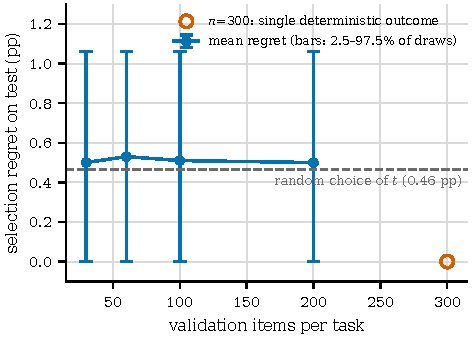
\includegraphics[width=\columnwidth]{figs/fig09b_val_size.pdf}
\caption{Test-set selection regret versus validation items per task. Solid markers: mean over 1000 random subsets, bars: 2.5--97.5\% of draws (the upper end is the worst grid point). Hollow marker at $n=300$: single deterministic realization, no interval. Dashed: regret of choosing $t$ at random.}
\label{fig:reg}
\end{figure}

\textbf{The point $n=300$.} Using the full pool involves no sampling. The selected coefficient is $t=0.7$ (validation macro $0.4961$, the largest of the 11), and the test optimum is also $t=0.7$ (macro $0.5090$). The regret is therefore $0$ and $P_{\mathrm{win}}=1$ because $0.5090$ exceeds both originals ($0.5025$ at $t=0$ and $0.5064$ at $t=1$). This is a coincidence of one realization. The subsets of $n=200$ contain two thirds of the pool and select $t=0.7$ in $198$ of 1000 draws, so the pool's own optimum anchors the large-$n$ end; the absence of a trend cannot be separated from the existence of a single pool of 300 items. The point has no interval, says nothing about the sampling variability of a 300-item validation set, and is not the endpoint of a trend from $0.50$ to $0$. The full-validation choice beats $t=0$ on test by $+0.65$~pp (paired bootstrap interval $[-0.23,+1.52]$; exploratory $p=0.149$). We detect no difference (the interval contains zero).

\textbf{Ties and random tie-breaking.} In the full pool the maximum is unique ($t=0.7$, $0.4961$), but four points tie just below it at $0.4953$ ($t=0,0.3,0.4,0.8$), and in subsets a tie at the maximum is common ($41.5$, $33.7$, $24.8$ and $28.4$\% of draws at $n=30,60,100,200$). With \texttt{np.argmax} the smallest tied $t$ wins (up to floating-point tolerance, Sec.~V), so $t=0$ is the most frequently selected point ($20$--$24$\% of draws), and $t=0$ has an above-average regret ($0.65$ versus $0.46$~pp for a random point). Breaking ties at random lowers the selection of $t=0$ to $14$--$20$\% and the mean regret to $0.47$, $0.50$, $0.48$ and $0.47$~pp (\texttt{results/summary\_art09\_random\_tiebreak.txt}). The bias toward $t=0$ therefore accounts for $0.02$--$0.03$~pp of the regret ($0.032$, $0.021$, $0.031$, $0.022$ at $n=30,60,100,200$) and contributes to the finding that regret is close to that of a random pick; with random ties the means are $0.01$--$0.04$~pp above the $0.46$~pp reference, and the conclusion of no detectable dependence on $n$ is unchanged.

\textbf{Flat curve, random baseline.} The test accuracies of the 11 points are $0.4983$ (min, $t=0.2$) to $0.5090$ (max, $t=0.7$): a range of $1.06$~pp, of the same order as the $0.76$~pp standard error of a single test accuracy. Regret is bounded by that range, so a mean of about $0.5$~pp is about half of the maximum possible loss ($0.47$--$0.50$ of the range). Picking a grid point at random loses $0.46$~pp. Four of $11$ grid points ($t=0.6,0.7,0.8,0.9$) beat both originals on test, a fraction of $0.36$, which is of the same order as the observed $P_{\mathrm{win}}$ of $0.31$--$0.37$ ($0.35$--$0.41$ with random tie-breaking; \texttt{results/summary\_art09\_random\_tiebreak.txt}). On this grid, validation selection at $n\le200$ is not clearly better than random choice in regret or in $P_{\mathrm{win}}$. The validation-based regrets ($0.50$--$0.53$~pp; $0.47$--$0.50$~pp with random ties) are slightly above the random $0.46$~pp.

\section{Discussion and Limitations}
The reading is narrow. On a grid whose test accuracies span $1.06$~pp, the regret is dominated by the flatness of the curve and is insensitive to $n$ from $30$ to $200$ items per task. All evaluations used bfloat16. Re-evaluating validation accuracy in fp32 at $t=0$, $0.7$ and $1$ lowered the macro accuracy by $0.67$, $0.41$ and $0.08$~pp (fp32: $0.4886$, $0.4920$, $0.4845$), a shift of the same size as the differences between coefficients, while the order of the three points did not change and WikiText-2 NLL moved by at most $0.0026$ nats at any $t$ (\texttt{results/fp32\_check\_qwen.txt}). Exact accuracy levels are therefore specific to bfloat16, and the test items were not re-evaluated in fp32. The validation set cannot tell apart candidates whose true differences are far below its resolution, and nothing it picks is far from the best. We conjecture that this is also why $P_{\mathrm{win}}$ is of the order of the random-choice fraction. We did not test this mechanism on other grids. A curve with a clear optimum would presumably show regret falling with $n$; this study contains no such curve, so it neither supports nor rules that out.

\textbf{Threats to validity.} (i) The pool is one realization. All subsets are drawn from the same 300 items without replacement, so they overlap (at $n=200$ each draw contains two thirds of the pool) and their spread underestimates the variation across independent validation sets. The pool's own optimum ($t=0.7$) also anchors the large-$n$ end of any curve ($198$ of 1000 draws select it at $n=200$), and the lack of trend cannot be separated from there being one pool of 300 items. (ii) The oracle $A^\ast$ is the maximum of 11 noisy test accuracies measured on the same test items used for scoring, so regret is measured against an optimistic reference. (iii) One model pair, one interpolation family, one hardware, four multiple-choice benchmarks, models of $\le0.5$B parameters; grids with more points or steeper curves are untested. (iv) Possible benchmark contamination was not examined. (v) The test split is easier than the validation split, which shifts levels but not regret definitions, because regret compares test accuracies only. (vi) ``Always $t=1$'' in Table~\ref{tab:reg} is a hindsight reference, not a selectable rule.

\section{Conclusion}
Among 11 interpolations of Qwen2.5-0.5B and its instruct variant, mean regret is $0.50$--$0.53$~pp for $30$ to $200$ validation items per task, with no detectable dependence on $n$. The probability of beating both originals ($0.31$--$0.37$) is of the same order as that of a random pick. The pre-registered expectation that regret falls with $n$ is not supported in this range, and the $n=300$ result is one deterministic coincidence that carries no weight. In the range $n=30$--$200$ on this grid, adding validation items does not change the expected regret, although the probability of zero regret roughly doubles (from $0.10$ to $0.20$ between $n=30$ and $200$); we do not extrapolate to larger pools or to other merge families. Random tie-breaking changes the means by $0.02$--$0.03$~pp and not the conclusion.

\section*{Data and Code Availability}
Repository \texttt{artigos-pesos-modelos-pequenos}, git tag \texttt{preprints-v1} (the commit that contains this manuscript and all scripts and caches); per-item cache in \texttt{cache/}. Original analysis: \texttt{experiments/analyze.py} (output \texttt{results/summary\_art09.txt}); added computations (test-curve range, random-choice regret, redraw, Fig.~\ref{fig:reg}): \texttt{experiments/an\_art0809\_extra.py} (output \texttt{results/summary\_art0809\_extra.txt}); random tie-breaking: \texttt{experiments/an\_art09\_random\_tiebreak.py} (seeds 0 and 3; output \texttt{results/summary\_art09\_random\_tiebreak.txt}). Single command: \texttt{./run\_everything.sh}. Software: Python 3.9.6, PyTorch 2.8.0, transformers 4.57.6, numpy 1.26.4, datasets 4.5.0; model revisions as in \texttt{MANIFEST.json}. Evaluation ran on Apple Silicon (MPS, bf16). No training is involved; seeds: split 0, subset draws 0, tie-break 3.

\section*{Acknowledgments}
No external funding.

\begin{thebibliography}{99}
\bibitem{miller2024errorbars} E.~Miller, ``Adding error bars to evals: A statistical approach to language model evaluations,'' arXiv:2411.00640, 2024.
\bibitem{gao2021lmeval} L.~Gao \emph{et al.}, ``EleutherAI/lm-evaluation-harness,'' Zenodo, doi:10.5281/zenodo.10256836.
\bibitem{clark2018arc} P.~Clark, I.~Cowhey, O.~Etzioni \emph{et al.}, ``Think you have solved question answering? Try ARC, the AI2 Reasoning Challenge,'' arXiv:1803.05457, 2018.
\bibitem{zellers2019hellaswag} R.~Zellers, A.~Holtzman, Y.~Bisk, A.~Farhadi, and Y.~Choi, ``HellaSwag: Can a machine really finish your sentence?'' in \emph{Proc.\ ACL}, 2019, arXiv:1905.07830.
\bibitem{sakaguchi2019winogrande} K.~Sakaguchi, R.~Le~Bras, C.~Bhagavatula, and Y.~Choi, ``WinoGrande: An adversarial Winograd schema challenge at scale,'' arXiv:1907.10641, 2019.
\bibitem{qwen2024qwen25} Qwen, A.~Yang \emph{et al.}, ``Qwen2.5 technical report,'' arXiv:2412.15115, 2024.
\bibitem{dwork2014adaptive} C.~Dwork, V.~Feldman, M.~Hardt \emph{et al.}, ``Preserving statistical validity in adaptive data analysis,'' arXiv:1411.2664, 2014.
\bibitem{recht2019imagenet} B.~Recht, R.~Roelofs, L.~Schmidt, and V.~Shankar, ``Do ImageNet classifiers generalize to ImageNet?'' arXiv:1902.10811, 2019.
\bibitem{efron1979bootstrap} B.~Efron, ``Bootstrap methods: Another look at the jackknife,'' \emph{Ann.\ Statist.}, vol.~7, no.~1, pp.~1--26, 1979, doi:10.1214/aos/1176344552.
\bibitem{wortsman2022soups} M.~Wortsman, G.~Ilharco, S.~Y. Gadre \emph{et al.}, ``Model soups: Averaging weights of multiple fine-tuned models improves accuracy without increasing inference time,'' in \emph{Proc.\ ICML}, 2022, arXiv:2203.05482.
\bibitem{rame2022ratatouille} A.~Ram\'e, K.~Ahuja, J.~Zhang \emph{et al.}, ``Model Ratatouille: Recycling diverse models for out-of-distribution generalization,'' arXiv:2212.10445, 2022.
\bibitem{rame2023rewarded} A.~Ram\'e, G.~Couairon, M.~Shukor \emph{et al.}, ``Rewarded soups: Towards Pareto-optimal alignment by interpolating weights fine-tuned on diverse rewards,'' arXiv:2306.04488, 2023.
\bibitem{ilharco2022taskarithmetic} G.~Ilharco, M.~T. Ribeiro, M.~Wortsman \emph{et al.}, ``Editing models with task arithmetic,'' in \emph{Proc.\ ICLR}, 2023, arXiv:2212.04089.
\bibitem{yadav2023ties} P.~Yadav, D.~Tam, L.~Choshen \emph{et al.}, ``TIES-Merging: Resolving interference when merging models,'' in \emph{Proc.\ NeurIPS}, 2023, arXiv:2306.01708.
\bibitem{akiba2024evolutionary} T.~Akiba, M.~Shing, Y.~Tang \emph{et al.}, ``Evolutionary optimization of model merging recipes,'' \emph{Nat.\ Mach.\ Intell.}, 2025, arXiv:2403.13187.
\bibitem{liu2024checkpointbo} D.~Liu, Z.~Wang, B.~Wang \emph{et al.}, ``Checkpoint merging via Bayesian optimization in LLM pretraining,'' arXiv:2403.19390, 2024.
\bibitem{matena2021fisher} M.~Matena and C.~Raffel, ``Merging models with Fisher-weighted averaging,'' arXiv:2111.09832, 2021.
\bibitem{yang2023adamerging} E.~Yang, Z.~Wang, L.~Shen \emph{et al.}, ``AdaMerging: Adaptive model merging for multi-task learning,'' in \emph{Proc.\ ICLR}, 2024, arXiv:2310.02575.
\bibitem{huang2023lorahub} C.~Huang, Q.~Liu, B.~Y. Lin \emph{et al.}, ``LoraHub: Efficient cross-task generalization via dynamic LoRA composition,'' in \emph{Proc.\ COLM}, 2024, arXiv:2307.13269.
\bibitem{yang2024survey} E.~Yang, L.~Shen, G.~Guo \emph{et al.}, ``Model merging in LLMs, MLLMs, and beyond: Methods, theories, applications and opportunities,'' arXiv:2408.07666, 2024.
\bibitem{santos2026modelmergingfo} D. F. Santos, ``Model Merging for Capability Composition: A Technical Note,'' Zenodo, 2026, doi:10.5281/zenodo.21610555.
\bibitem{santos2026collapseresist} D. F. Santos, ``Collapse-Resistant Joint-Embedding Predictive Architectures: A Controlled Comparison of SIGReg, VICReg, and EMA,'' Zenodo, v2, 2026, doi:10.5281/zenodo.24223364.
\bibitem{santos2026knowledgedisti} D. F. Santos, ``Knowledge Distillation and Self-Distillation for Language Models,'' Zenodo, 2026, doi:10.5281/zenodo.21610100.
\bibitem{santos2026parametereffic} D. F. Santos, ``Parameter-Efficient Fine-Tuning: LoRA, QLoRA, and DoRA,'' Zenodo, 2026, doi:10.5281/zenodo.21610033.
\bibitem{santos2026mixtureofexper} D. F. Santos, ``Mixture-of-Experts Training and Sparse Upcycling,'' Zenodo, 2026, doi:10.5281/zenodo.21610062.
\bibitem{santos2026curriculumlear} D. F. Santos, ``Curriculum Learning and Data-Efficient Pretraining: A Technical Note,'' Zenodo, 2026, doi:10.5281/zenodo.21610595.
\bibitem{santos2026syntheticdatag} D. F. Santos, ``Synthetic Data Generation and Self-Improvement: A Technical Note,'' Zenodo, 2026, doi:10.5281/zenodo.21610525.
\bibitem{santos2026directpreferen} D. F. Santos, ``Direct Preference Optimization (DPO): A Technical Note,'' Zenodo, 2026, doi:10.5281/zenodo.21609911.
\end{thebibliography}

\end{document}
